%!TEX root = ../MasterThesis.tex

\section{An overview of \gls{E-commerce}}
\label{sec:e_commerce_scenario}

\gls{E-commerce} as a term relates to the trading of products or services utilizing a computer network such as the Internet. It is usually categorized into the following four different subfields \citep{sen2015study}:\@

\begin{enumerate}
  \item \textbf{Business-To-Business (\gls{B2B})}: refers to electronic trading between companies with the objective to improve their supply chain processes
  \item \textbf{Business-To-Consumer (\gls{B2C})}: refers to electronic trading between a company and its consumers (most publicly known example for it is Amazon \citep{Amazon.com})
  \item \textbf{Consumer-To-Consumer (\gls{C2C})}: refers to electronic trading between consumers (most publicly known example for that is eBay \citep{eBayInc})
  \item \textbf{Consumer-To-Business (\gls{C2B})}: refers to electronic trading between consumers and businesses (most publicly known example for this is TaskRabbit \citep{TaskRabbit})
\end{enumerate}

This Master thesis will \textbf{\underline{solely}} focus on the \gls{B2C} aspect of \gls{E-commerce}. In that case a consumer is using an \gls{E-commerce} shop of a merchant on the Internet to order products or services online. The merchant is offering a catalog of available products or services on the Web, that is available and accessible by the general public and usually has a nation-wide if not global reach. The merchant can either run the \gls{E-commerce} shop software on their own servers (on-premise) or can outsource this additional sales channel to a 3$^{rd}$ party hosting company or cloud service provider (\gls{CSP}). Also the \gls{E-commerce} shop software itself can be either developed by the merchant in-house or acquired as a boxed product from an Independent Software Vendor (\gls{ISV}) on the market. For business accounting purposes the merchant also runs a bank account with the acquirer (see Figure~\ref{fig:images_ecommerce_scenario}). \\

When placing an order with the merchant online, the consumer is usually using a credit card for finalizing the transaction. This credit card has originally been handed out by the issuing bank to the consumer. Additionally, in some online shops it is mandatory for the consumer to create an user account with them, while in others it is not. The former is the preferred way when consumers are repetitively buying from that merchant, whereas the latter might be used for one-time or irregular shopping trips online. To be able to connect to the Internet the consumer also relies on a service of an Internet Service Provider (\gls{ISP}). The whole initial setup for participating on \gls{E-commerce} activities is found in Figure~\ref{fig:images_ecommerce_scenario}.\@

\begin{figure}[H]
	\centering
		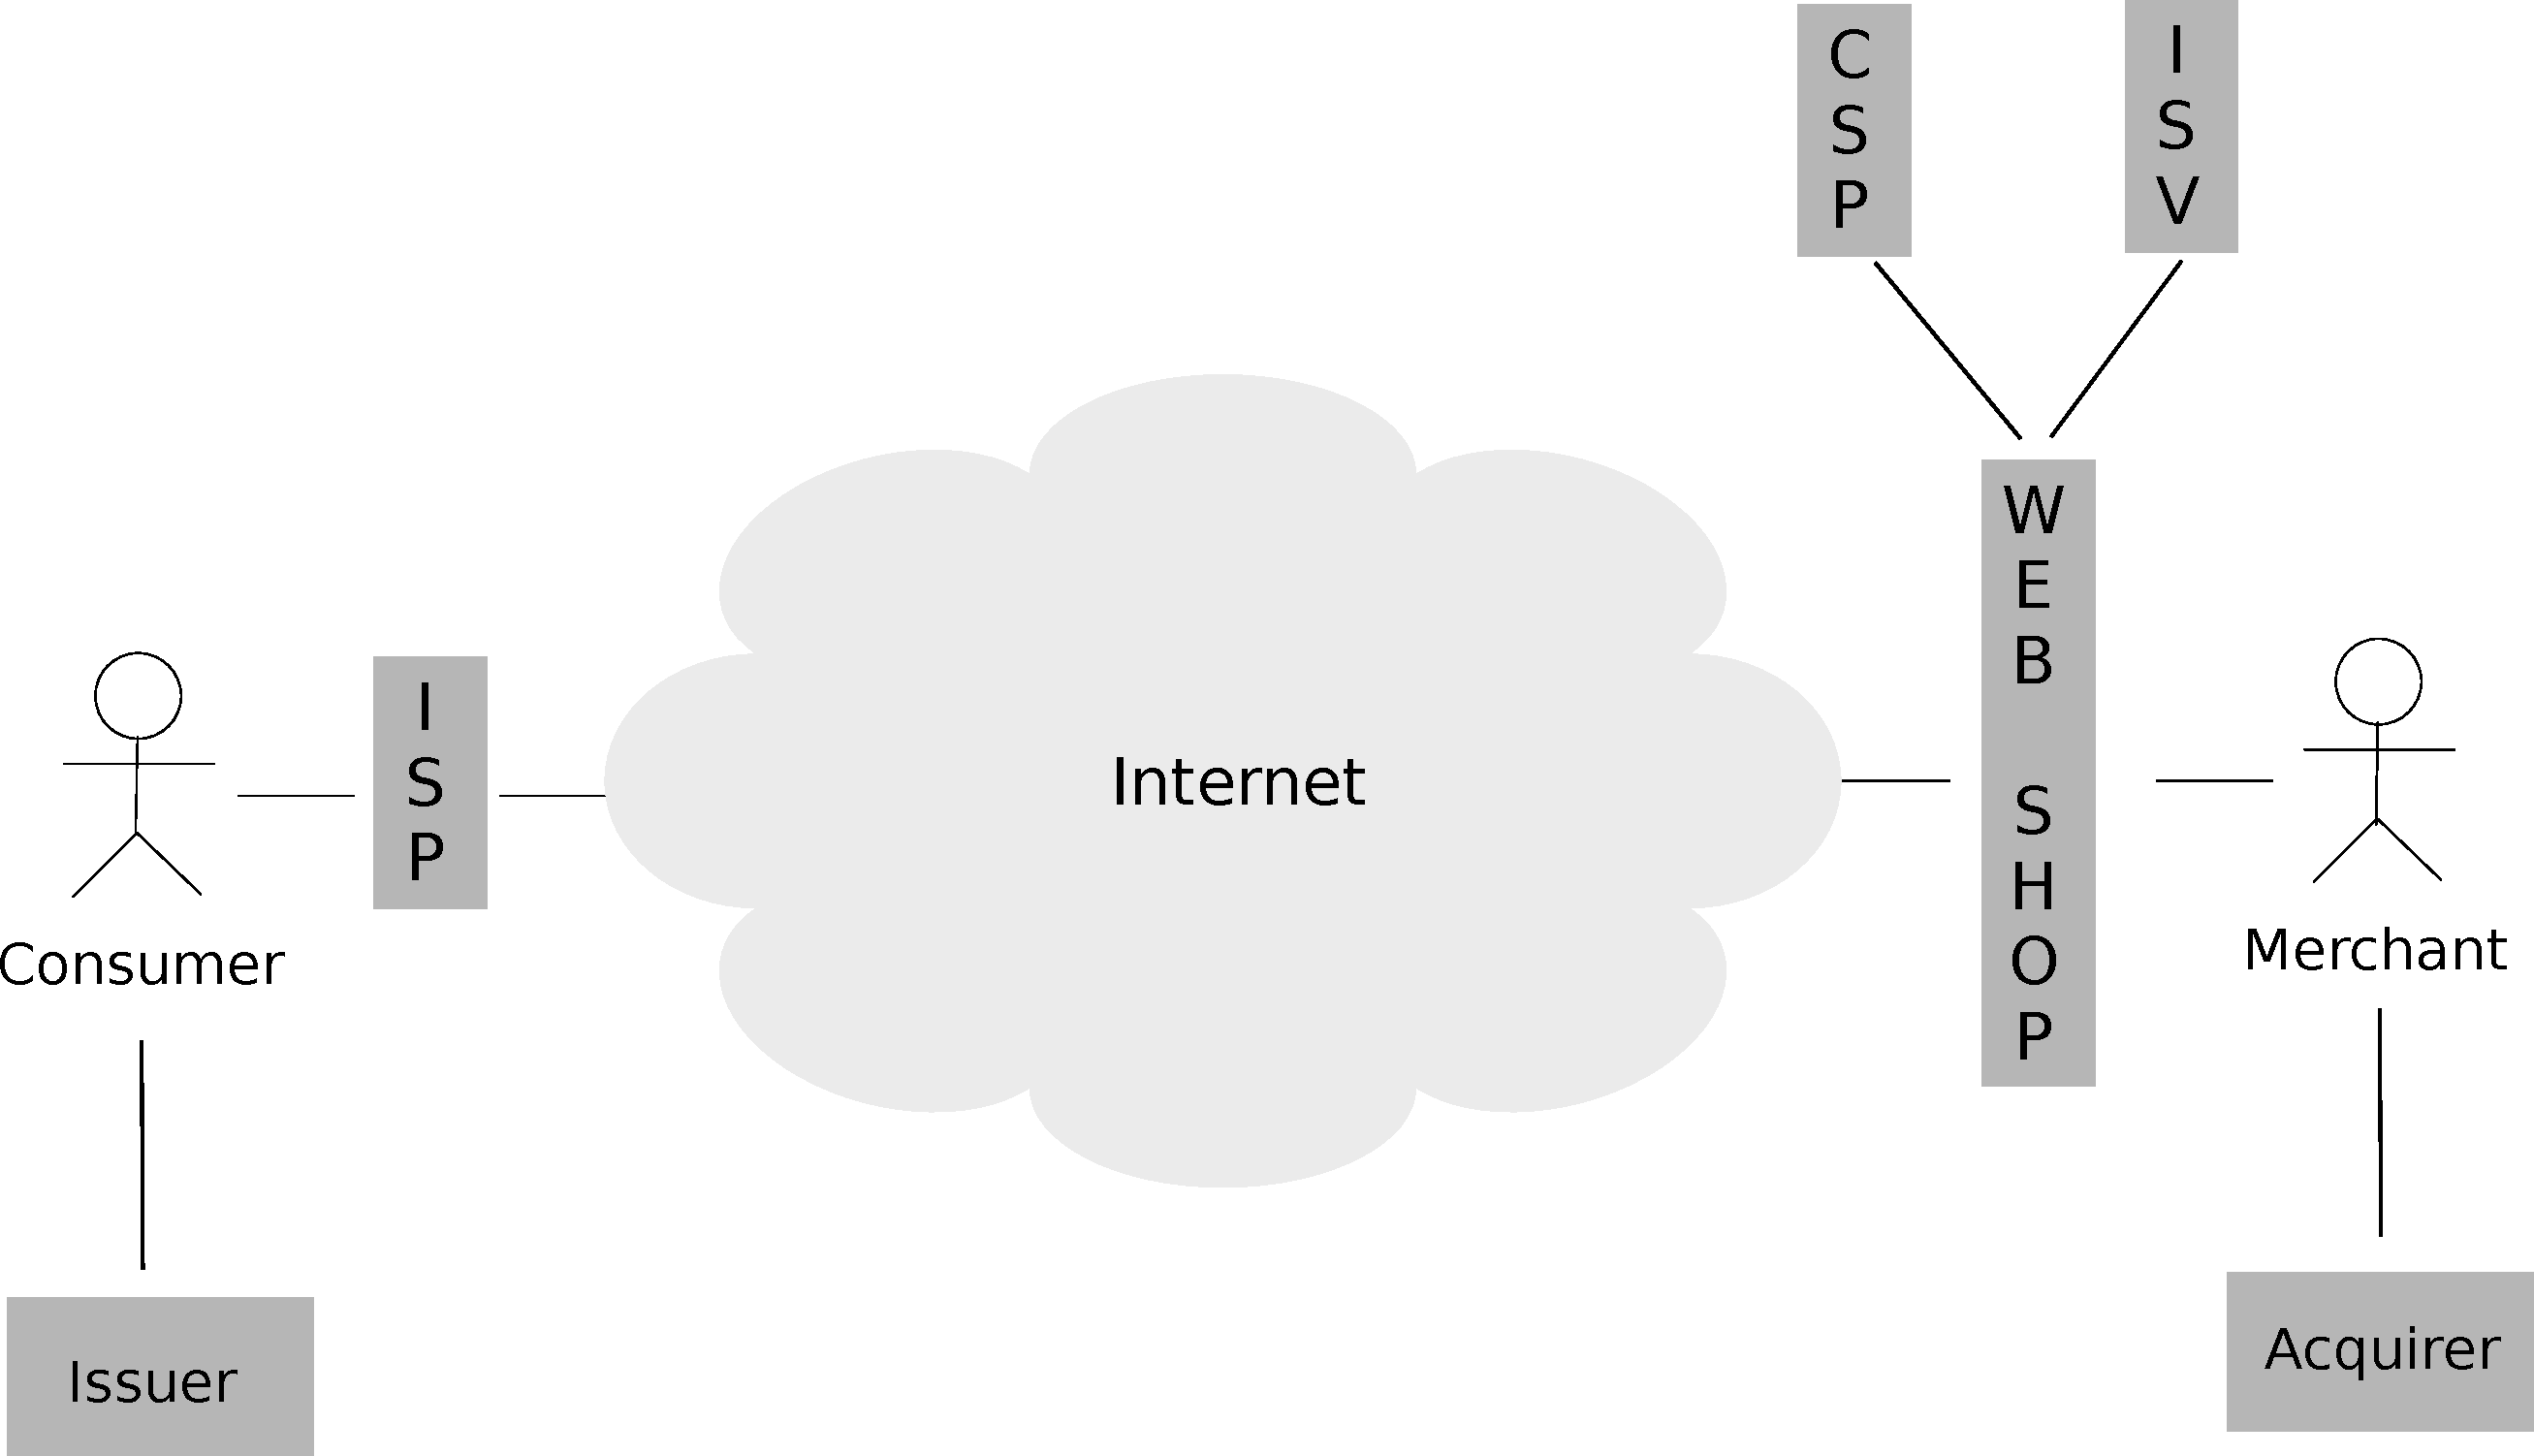
\includegraphics[width=0.9\columnwidth]{images/e-commerce-scenario.pdf}
	\caption{\gls{E-commerce} Fundamentals}
\label{fig:images_ecommerce_scenario}
\end{figure}

When the consumer places the order online, the merchant receives at least a list of products or services from the current shopping cart of the consumer, the identification of the consumer as well as the delivery address to ship the physical items to. If the transaction is going to be finalized with a credit card, the consumer will have to provide additional information like their billing address and credit card information (including the id, the expiry date and the security number of the card). \\

The merchants usually doe not validate the credit card information on their own. For that purpose they are relying on another 3$^{rd}$ party service offered on the Internet by the Payment Service Provider (\gls{PSP}). These providers are either validating the credit card information themselves based on an user profile the consumer has with the \gls{PSP} (e.g.\ a globally available Web service such as PayPal), or are connecting to the issuing bank of the credit card for doing so. For initiating this validation process the merchant is handing over the billing information to the \gls{PSP} incl.\ the credit card information given by the consumer. \\

Either the \gls{PSP} or the issuing bank is validating the correctness of these information with criterias like: \@

\begin{itemize}
    \item is the billing address matching the current consumers' postal address on file?
    \item is the stated credit card information correct?
    \item is the credit card still valid?
    \item is the credit card not marked as being blocked in the internal databases?
\end{itemize}

The merchant will receive the status of the authorization as well as an unique payment token in return. If the authorization was done successfully, the merchant will collect the items and send out a shipping request to one of the available Logistic Service Providers (\gls{LSP}), that are capable to handle the delivery of the order. They will pickup the items at the merchant's facility and ship them to the delivery address stated by the consumer. Usually in parallel the merchant is informing their bank about the order, amount due as well as the payment token received from the \gls{PSP}. The acquirer is in charge to withdrawal the amount of the order from the consumer's bank account either via the \gls{PSP} or directly from the issuing bank, depending on who of them has authorized the initial payment request (a process called clearing) \citep{VisaPayment2014}. The sequence of activities within an \gls{E-commerce} checkout process is visualized in Figure~\ref{fig:images_ecommerce_checkout_process}.\@

\begin{figure}[!ht]
	\centering
		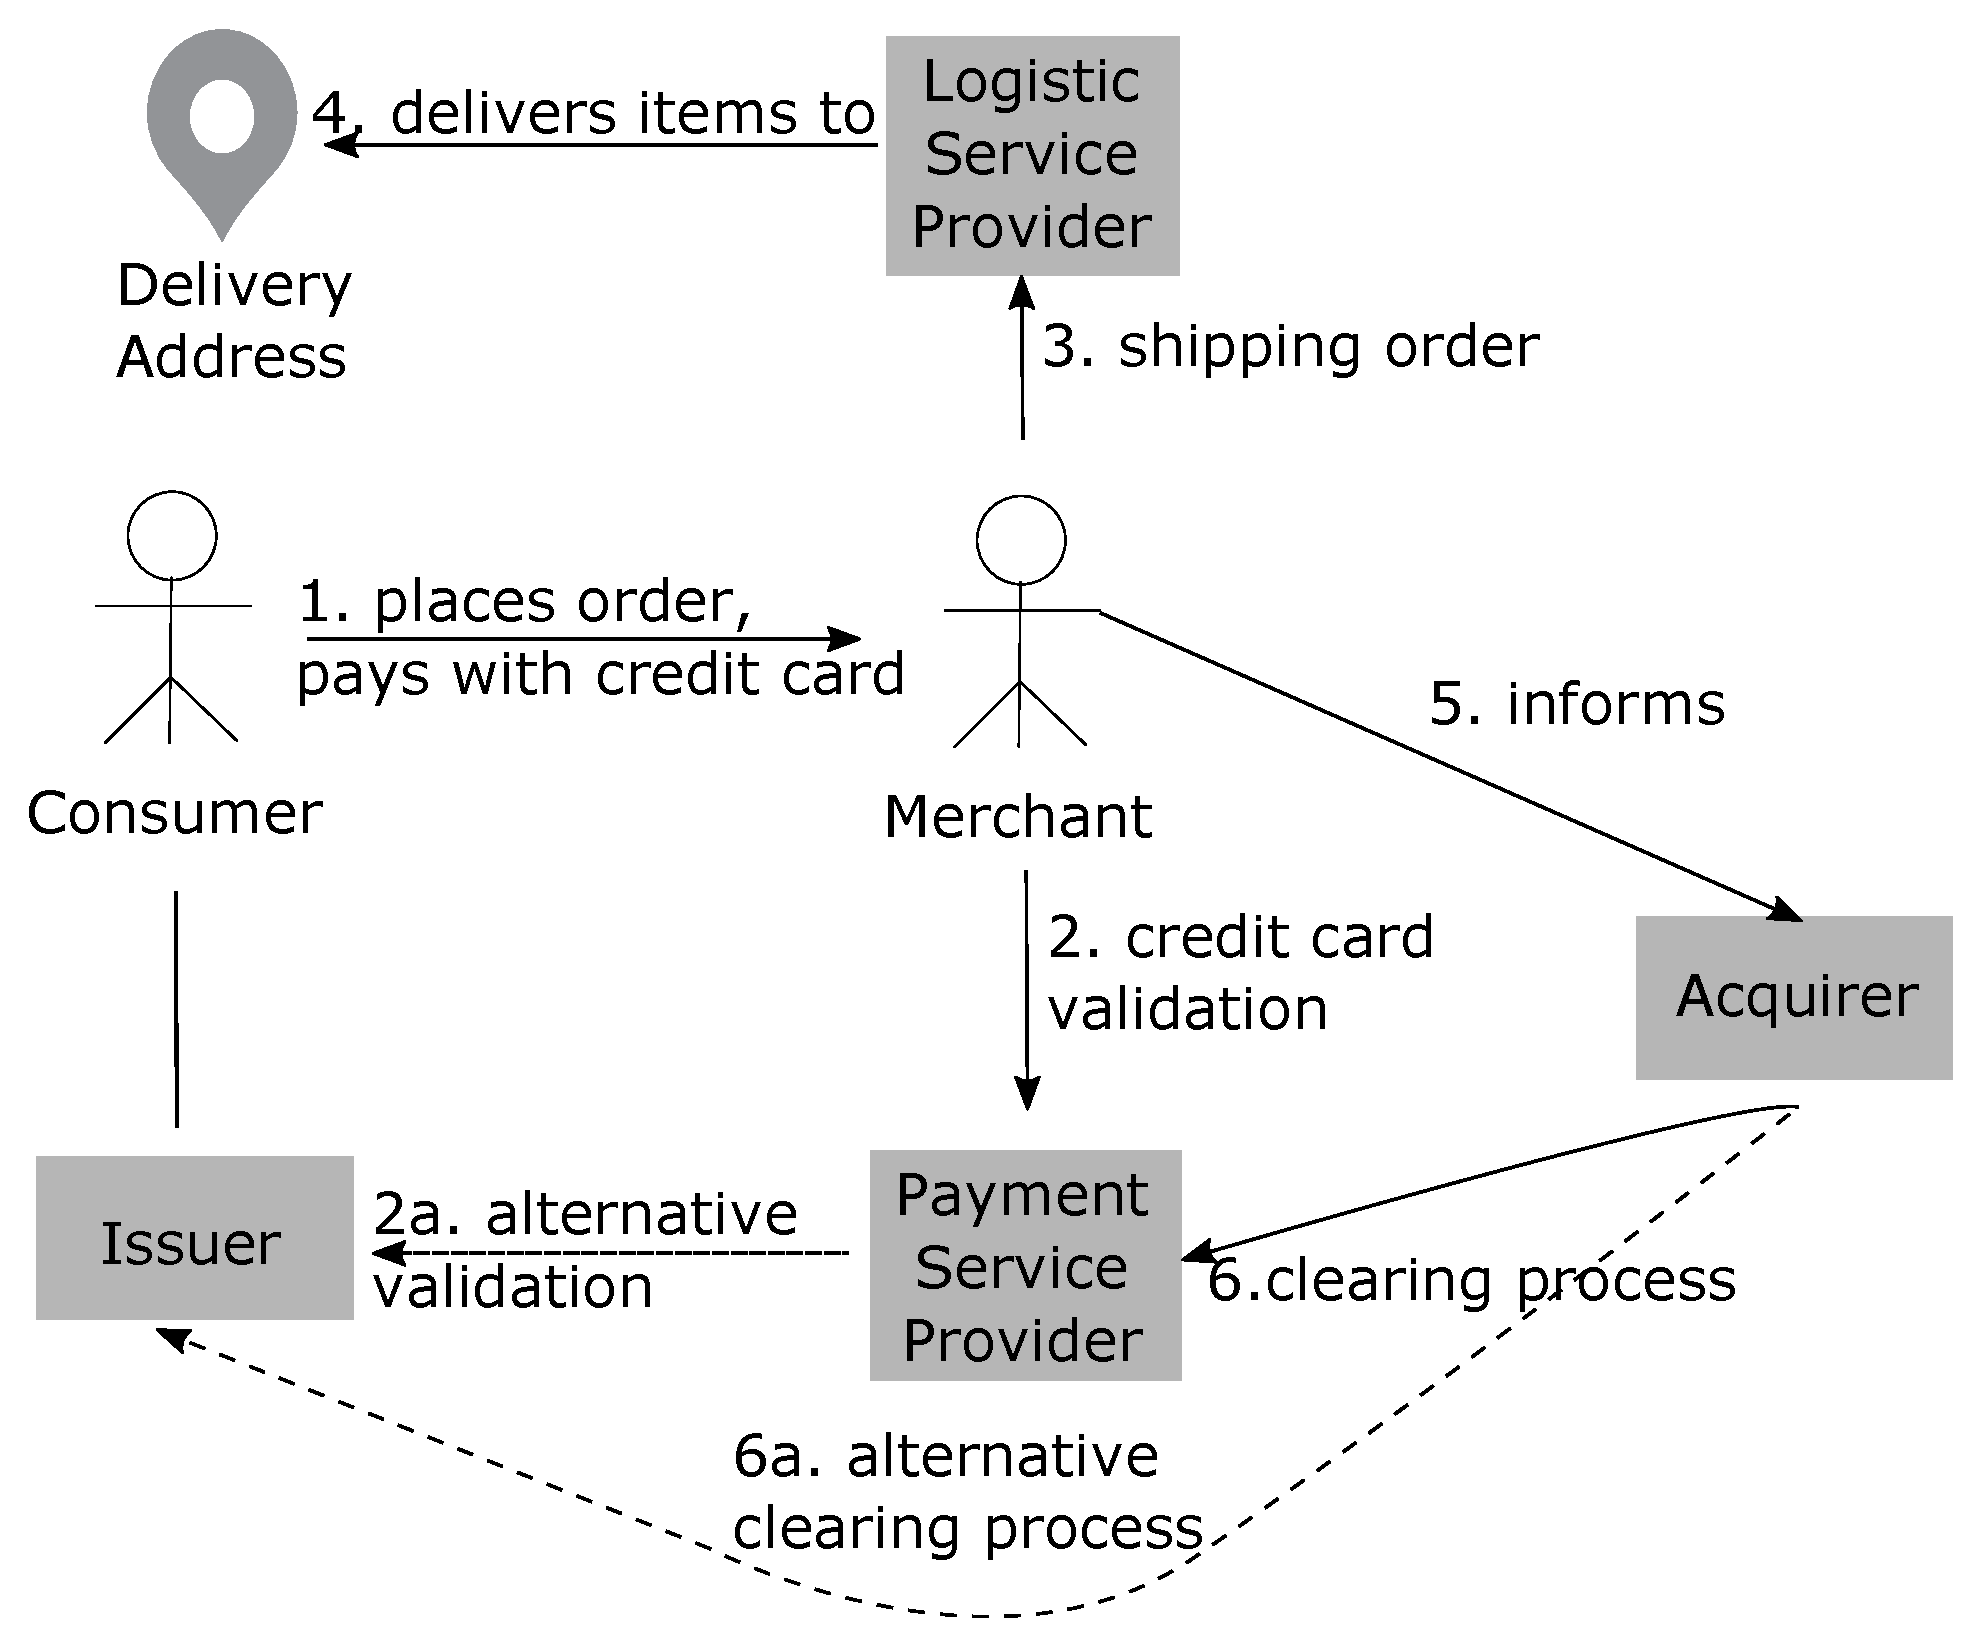
\includegraphics[width=0.9\columnwidth]{images/e-commerce-checkout-process.pdf}
	\caption{\gls{E-commerce} Checkout Process in detail}
\label{fig:images_ecommerce_checkout_process}
\end{figure}

% section scenario description (end)
